The \textit{Experiment Management Service} module is responsible for monitoring the running
program and gathering data from the instance and generate data, and send it to
the web client for reporting. The monitor will record data such as CPU time,
CPU usage, RAM usage, Network throughput, Overall running time, etc.
\\
\\
The Experiment Management service then will delete the instance of the running program them
send the data collected to the web serve in order for it to be processed so a
report can be generated. It will store the data in a database. When the benchmarking
is complete, the system will use the notifiaction system to notify the client their
benchmark is complete.


\subsection{Scope}
The scope for the Experiment Management Service module is shown in Figure \ref{Benchmark Scope}
\begin{figure}[H]
  \begin{center}
  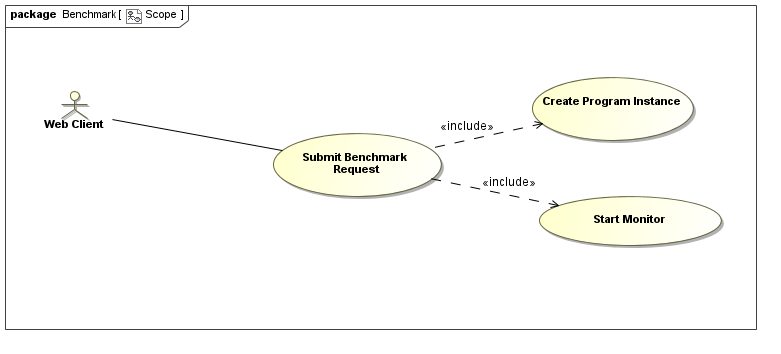
\includegraphics[scale=0.5]{../Diagrams and Charts/Benchmark/Scope.png}
  \caption{Experiment Management Scope}
  \end{center}
  \label{Benchmark Scope}
\end{figure}
The scope of the Experiment Management Service module include:
\begin{itemize}
	\item Receive a program to run.
  \item Monitor the program instance
  \item Record data
  \item Generate server data for reporting, using the Reporting Module
  \item Store data in database
\end{itemize}

\subsection{Domain Model}
The domain model for the Experiment Management Service module is shown in Figure \ref{Benchmark Domain Model}
\begin{figure}[H]
  \begin{center}
  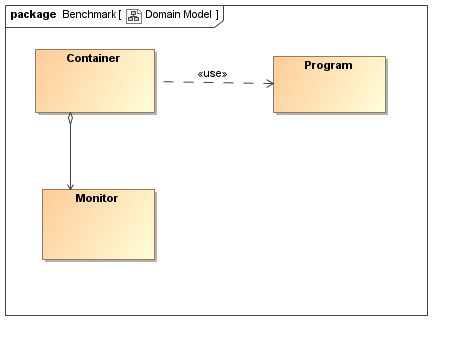
\includegraphics[scale=1.0]{../Diagrams and Charts/Benchmark/Domain Model.png}
  \caption{Experiment Management Domain Model}
  \end{center}
  \label{Benchmark Domain Model}
\end{figure}
There will be a container which contains the program to be run, and the monitor to monitor the program instance.\\
